\documentclass[journal]{IEEEtran}

\usepackage{amsmath,amssymb}
\usepackage{array}
\usepackage{booktabs}
\usepackage{cite}
\usepackage{graphicx}
\usepackage{multirow}
\usepackage{tikz}
\usetikzlibrary{arrows.meta,positioning,shapes.geometric}
\usepackage[hidelinks]{hyperref}
\usepackage{xcolor}

\title{Event-TimeRAF: Event-Aware Retrieval-Augmented Foundation Models for Explainable Air Quality Forecasting Under Concept Drift}

\author{Author Name,~\IEEEmembership{Student Member,~IEEE}%
\thanks{This manuscript reports an academic Kaggle-based experiment using official-source public data.}
}

\begin{document}

\maketitle

\begin{abstract}
Urban air-quality forecasting is important for public-health warnings, environmental management, and city-scale decision support. Recent time-series foundation models have shown useful zero-shot forecasting capability, and TimeRAF enriches such models by retrieving relevant time-series sequences from a knowledge base and incorporating them into a frozen time-series foundation model. However, air-pollution variation is often influenced by outside context, including meteorology, holidays, wildfire smoke, high-wind events, heavy rain, and other environmental factors. This paper presents Event-TimeRAF, an event-aware retrieval-augmented forecasting framework for Los Angeles County PM2.5 prediction. The framework combines historical air-quality windows, weather features, calendar context, retrieved time-series patterns, source-recorded environmental events, distribution-shift indicators, and evidence-based explanation generation. We evaluate the method on official EPA AirData PM2.5 observations, NOAA Global Hourly weather, and hash-verified NOAA Storm Events records for 2019--2024. In the final Kaggle run, the best overall model is the weather-calendar XGBoost context baseline with MSE 26.185, while the full Event-TimeRAF XGBoost variant obtains MSE 26.712. The frozen Chronos-Bolt baseline obtains MSE 28.941, and retrieval-augmented Chronos improves it to MSE 28.709. Because NOAA Storm Events lacks machine-readable publication timestamps, event-aware results are reported as retrospective event-start sensitivity results rather than strict real-time event forecasts.
\end{abstract}

\begin{IEEEkeywords}
Air quality forecasting, PM2.5, retrieval-augmented forecasting, time-series foundation models, TimeRAF, concept drift, explainable forecasting.
\end{IEEEkeywords}

\section{Introduction}

Air pollution is a major urban risk factor, and fine particulate matter (PM2.5) is especially important because of its association with respiratory and cardiovascular health impacts \cite{who2021airquality}. Forecasting PM2.5 can support public-health alerts, exposure reduction, transport planning, and environmental policy. In dense cities such as Dhaka, air quality can vary rapidly because of meteorological conditions, traffic patterns, seasonal effects, construction dust, industrial activity, and abnormal events. These characteristics make air-quality forecasting a challenging time-series forecasting problem.

Classical forecasting models and machine-learning models such as ARIMA, tree-based regressors, recurrent neural networks, and Transformer-based models can capture historical patterns when training and testing conditions are similar. However, urban air quality is highly context-dependent. A model trained only on historical numerical trends may underperform during unusual weather, public holidays, traffic disruptions, fire incidents, dust events, or other external shocks. This limitation is closely related to concept drift, where the data-generating process changes over time.

Time-series foundation models (TSFMs) have recently been proposed to improve generalization across forecasting tasks. Models such as TimesFM, Moirai, MOMENT, Chronos, and Tiny Time Mixers (TTM) aim to transfer forecasting knowledge learned from large time-series corpora to new downstream domains \cite{das2024timesfm,woo2024moirai,goswami2024moment,ansari2024chronos,ekambaram2024ttm}. TimeRAF extends this direction by introducing retrieval augmentation for zero-shot time-series forecasting \cite{zhang2025timeraf}. It builds a time-series knowledge base, retrieves relevant candidate sequences, and integrates retrieved knowledge using Channel Prompting while keeping the TSFM backbone frozen.

Although TimeRAF is a strong base method, its retrieval knowledge is primarily numerical time-series data. For air-quality forecasting, external context is not optional: rainfall can wash out particulates, low wind speed can increase stagnation, holidays can change traffic patterns, and fire or construction events can introduce abrupt emission changes. Therefore, a natural extension is to retrieve not only similar time-series patterns but also event, weather, and calendar context relevant to the forecast horizon.

This draft proposes Event-TimeRAF, an event-aware retrieval-augmented framework for explainable Dhaka PM2.5 forecasting under concept drift. The planned contributions are:
\begin{itemize}
    \item an event-aware retrieval-augmented forecasting framework for urban PM2.5 prediction;
    \item a hybrid knowledge-base design combining air-quality windows, weather summaries, calendar context, and event/news records;
    \item a TimeRAF-inspired retrieval baseline using random and similarity-based retrieval over historical windows;
    \item simple concept-drift indicators based on distribution shift, retrieval similarity, weather changes, and event bursts;
    \item evidence-based explanation generation using retrieved historical cases, event context, weather drivers, drift indicators, and feature importance;
    \item a planned ablation study comparing no retrieval, random retrieval, time-series retrieval, event retrieval, drift-aware retrieval, and the full Event-TimeRAF framework.
\end{itemize}

This manuscript is intentionally written as a draft before implementation. Sections on results and discussion contain only the reporting plan and placeholders. No experimental performance values are fabricated.

\section{Literature Review and Related Work}

\subsection{Statistical, Machine-Learning, and Deep Forecasters}
Forecasting methods differ in how they trade inductive bias, data demand, and
computational cost. Autoregressive and seasonal models remain informative
baselines because their failure modes are easy to inspect. Tree ensembles such
as XGBoost and LightGBM extend this setting to nonlinear lag, rolling, weather,
and calendar interactions without requiring a sequence encoder
\cite{chen2016xgboost,ke2017lightgbm}. Recurrent LSTM and GRU models instead
learn stateful temporal representations \cite{hochreiter1997lstm,cho2014gru}.
Large benchmark archives, including the Monash Forecasting Repository, further
support reproducible comparison across heterogeneous time-series domains
\cite{godahewa2021monash}.
Transformer families emphasize longer dependencies: Informer reduces attention
cost, Autoformer and FEDformer use decomposition, Crossformer and iTransformer
model cross-variable structure, and TimesNet reorganizes temporal variation
into two-dimensional patterns
\cite{zhou2021informer,wu2021autoformer,zhou2022fedformer,zhang2023crossformer,liu2024itransformer,wu2023timesnet}.
These gains do not imply that greater architectural complexity is always
necessary. DLinear and PatchTST show that simple decomposition or patch-based
inductive biases can remain highly competitive \cite{zeng2023dlinear,nie2023patchtst},
whereas TimeMixer uses explicit multiscale decomposition and mixing
\cite{wang2024timemixer}. Event-TimeRAF therefore retains seasonal and boosted
tree baselines instead of treating a deep backbone as the default winner.

\subsection{Time-Series Foundation Models}
Time-series foundation models (TSFMs) seek transfer across datasets rather than
training a separate representation from scratch for each series. TimesFM uses a
decoder-only forecasting design; Moirai trains a universal forecasting
Transformer; MOMENT supports several time-series tasks; Chronos represents
values as tokens; and Tiny Time Mixers emphasizes compact zero- and few-shot
transfer
\cite{das2024timesfm,woo2024moirai,goswami2024moment,ansari2024chronos,ekambaram2024ttm}.
Timer, Timer-XL, UniTime, and Time-LLM explore generative pretraining,
long-context scaling, cross-domain unification, or language-model reprogramming
\cite{liu2024timer,liu2025timerxl,liu2024unitime,jin2024timellm}. Frozen
pretrained models have also been evaluated as general computation engines for
time-series analysis \cite{zhou2023onefitsall}. Collectively, these studies
motivate zero-shot evaluation, but they also show that transfer performance
depends on input representation and domain shift. The present study therefore
compares frozen Chronos-Bolt against locally supervised models on identical
forecast origins rather than assuming foundation-model superiority.

\subsection{Retrieval-Augmented Forecasting}
Retrieval augmentation separates parametric knowledge from an external memory.
In natural-language processing, RAG and Dense Passage Retrieval established the
retrieve-then-condition pattern \cite{lewis2020rag,karpukhin2020dpr}. In time
series, retrieval has been studied through diffusion forecasting and assisted
generation workflows \cite{liu2024ratd,ang2024tsgassist}. TimeRAF provides the
closest methodological reference: it constructs a time-series knowledge base,
trains an MLP dual-encoder retriever, selects top-$k$ candidates, and integrates
candidate embeddings into a frozen TSFM through Channel Prompting
\cite{zhang2025timeraf}. Its ablations separate retrieval quality, integration,
candidate count, knowledge-base composition, and backbone choice.

Event-TimeRAF retains the external-memory principle but addresses a different
experimental question. It uses transparent random, cosine, and event-context
similarity instead of a learned dual encoder, and it uses feature- or
forecast-level fusion instead of internal Channel Prompting. This distinction
prevents the current implementation from being described as a reproduction of
TimeRAF; it is an audited environmental adaptation designed to test whether
contextual historical analogues help a local PM2.5 task.

\subsection{Air-Quality Forecasting and Official Context}
PM2.5 forecasting commonly combines pollutant history with temperature,
humidity, wind, precipitation, and pressure. Recent reviews describe a shift
from single-station recurrent models toward attention-based, hybrid, and
spatiotemporal systems \cite{zhou2024pm25review,zhang2023sparsepm25}. AirFormer,
for example, separates deterministic spatiotemporal modeling from stochastic
uncertainty estimation at nationwide scale \cite{liang2023airformer}. Such
multi-station designs address spatial dependence, whereas the present study
examines a county-level aggregate and the provenance of contextual evidence.
EPA AirData supplies regulated PM2.5 observations, NOAA Integrated Surface
Database supplies hourly meteorology, and NOAA Storm Events supplies structured
hazard records \cite{epaairdata2026,noaaisd2026,noaastormevents2026}. NOAA
Hazard Mapping System products could add smoke evidence but were not included in
the reported run \cite{noaahms2026}.

\subsection{Distribution Shift and Forecast Explanations}
Temporal nonstationarity can alter means, variances, and relationships between
inputs and future values. Adaptive normalization methods address this problem by
estimating statistics at local temporal scales \cite{liu2023san}; Event-TimeRAF
instead uses interpretable shift indicators to audit regimes without claiming
that shift has been eliminated. Explanation methods also differ in scope. SHAP
attributes predictions to model inputs \cite{lundberg2017shap}, while
information-theoretic saliency supports counterfactual inspection of
probabilistic forecasts \cite{raman2023forecast}. The implemented explanation
layer is narrower: it records signed XGBoost effects, retrieved cases, event
identifiers, drift components, and an uncertainty proxy. These records support
traceability, but they do not establish causal effects of weather or events.

\section{Problem Formulation}

Let $x_t$ denote the PM2.5 measurement at time $t$. For a forecast time $t$, the historical air-quality lookback window is
\begin{equation}
    X_t = [x_{t-L+1}, x_{t-L+2}, \ldots, x_t],
    \label{eq:lookback}
\end{equation}
where $L$ is the lookback length. Let $W_t$ denote weather covariates aligned
with the lookback window, $C_t$ denote calendar features, and $E_t$ denote event
context available under the recorded source assumption at the forecast origin.
The target associated with the input in (\ref{eq:lookback}) is
\begin{equation}
    Y_{t+1:t+H} = [x_{t+1}, x_{t+2}, \ldots, x_{t+H}],
    \label{eq:target}
\end{equation}
where $H$ is the forecasting horizon.
Equation~(\ref{eq:target}) therefore defines the 24-step vector evaluated at
every valid origin.

The forecasting goal is to learn a function
\begin{equation}
    \hat{Y}_{t+1:t+H} =
    F_{\theta}(X_t, W_t, C_t, E_t, R^{ts}_t, R^{ev}_t, D_t),
    \label{eq:forecast}
\end{equation}
where $R^{ts}_t$ is retrieved time-series knowledge, $R^{ev}_t$ is retrieved event knowledge, and $D_t$ contains concept-drift indicators. The implemented target setting is $L=168$ hours and $H=24$ hours.
Equation~(\ref{eq:forecast}) states the full information interface; the
implemented modules that construct these arguments are specified in the next
section.

The evaluation uses a time-based split:
\begin{equation}
    \mathcal{T}_{train} < \mathcal{T}_{val} < \mathcal{T}_{test},
    \label{eq:chronological_split}
\end{equation}
where the earliest 70\% of observations are used for training, the next 15\%
for validation, and the latest 15\% for testing. The ordering in
(\ref{eq:chronological_split}) is retained for feature fitting, retrieval
eligibility, model selection, and final evaluation.

Table~\ref{tab:symbols} summarizes the essential notation.

\begin{table}[!t]
\centering
\caption{Main Symbols Used in the Proposed Formulation}
\label{tab:symbols}
\begin{tabular}{ll}
\toprule
Symbol & Meaning \\
\midrule
$L$ & Lookback window length \\
$H$ & Forecast horizon \\
$X_t$ & Historical PM2.5 sequence at time $t$ \\
$W_t$ & Weather covariates \\
$C_t$ & Calendar/context features \\
$E_t$ & Event context available at the forecast origin \\
$R^{ts}_t$ & Retrieved time-series knowledge \\
$R^{ev}_t$ & Retrieved event knowledge \\
$D_t$ & Drift indicators \\
$q_t$ & SACB context vector in $\mathbb{R}^{86}$ \\
$G_t$ & LSER top-$k$ retrieved set \\
$\rho(G_t)$ & Retrieval summary in $\mathbb{R}^{51}$ \\
$\mathcal{O}_t$ & Machine-readable DFEH evidence record \\
$\hat{Y}_{t+1:t+H}$ & Predicted future PM2.5 values \\
\bottomrule
\end{tabular}
\end{table}

\section{Methodology}

\subsection{Overview}
Fig.~\ref{fig:architecture} shows the planned Event-TimeRAF pipeline. The system first aligns air-quality observations with weather and calendar features. It then constructs sliding windows and a time-series knowledge base. A time-series retriever returns similar historical windows, while an event retriever returns relevant event/news records around the forecast timestamp. Retrieved evidence is fused with structured features to generate a forecast, confidence proxy, drift score, and explanation.

\begin{figure}[!t]
\centering
\resizebox{\columnwidth}{!}{%
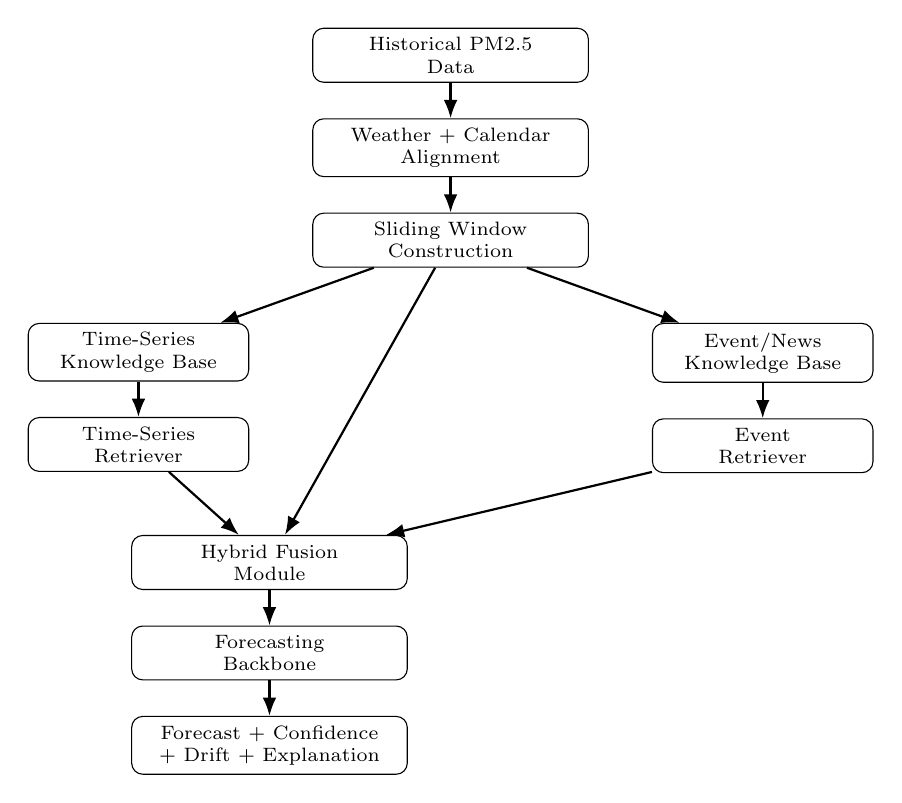
\begin{tikzpicture}[
    node distance=4.5mm,
    block/.style={rectangle, rounded corners, draw=black, align=center, minimum width=35mm, minimum height=6mm, font=\scriptsize},
    smallblock/.style={rectangle, rounded corners, draw=black, align=center, minimum width=28mm, minimum height=6mm, font=\scriptsize},
    arrow/.style={-Latex, thick}
]
\node[block] (air) {Historical PM2.5\\Data};
\node[block, below=of air] (align) {Weather + Calendar\\Alignment};
\node[block, below=of align] (windows) {Sliding Window\\Construction};
\node[smallblock, below left=7mm and 8mm of windows] (tskb) {Time-Series\\Knowledge Base};
\node[smallblock, below right=7mm and 8mm of windows] (evkb) {Event/News\\Knowledge Base};
\node[smallblock, below=of tskb] (tsret) {Time-Series\\Retriever};
\node[smallblock, below=of evkb] (evret) {Event\\Retriever};
\node[block, below right=8mm and -15mm of tsret] (fusion) {Hybrid Fusion\\Module};
\node[block, below=of fusion] (model) {Forecasting\\Backbone};
\node[block, below=of model] (out) {Forecast + Confidence\\+ Drift + Explanation};

\draw[arrow] (air) -- (align);
\draw[arrow] (align) -- (windows);
\draw[arrow] (windows) -- (tskb);
\draw[arrow] (windows) -- (evkb);
\draw[arrow] (tskb) -- (tsret);
\draw[arrow] (evkb) -- (evret);
\draw[arrow] (windows) -- (fusion);
\draw[arrow] (tsret) -- (fusion);
\draw[arrow] (evret) -- (fusion);
\draw[arrow] (fusion) -- (model);
\draw[arrow] (model) -- (out);
\end{tikzpicture}
}
\caption{Planned Event-TimeRAF architecture. The figure is conceptual and does not report experimental results.}
\label{fig:architecture}
\end{figure}

\subsection{Relationship to TimeRAF}
TimeRAF retrieves top-$k$ candidate time-series windows from a curated knowledge base and integrates retrieved candidates using Channel Prompting \cite{zhang2025timeraf}. It uses a learnable dual-encoder retriever, dot-product similarity, a frozen TSFM backbone, and candidate augmentation during retriever training. Event-TimeRAF preserves the retrieval-augmentation principle but adapts it to Dhaka PM2.5 forecasting and expands the knowledge sources beyond numerical sequences.

The first implementation will not reproduce full TimeRAF. Instead, it will implement a TimeRAF-inspired retrieval baseline using random retrieval and cosine similarity. A dual-encoder MLP retriever, candidate augmentation, and TSFM-based Channel Prompting are reserved for later extensions after the Kaggle-compatible MVP is reproducible.

\subsection{Dataset Construction}
The planned air-quality data source is OpenAQ or another accessible source containing Dhaka PM2.5 observations. Timestamps will be converted to Asia/Dhaka time, resampled to hourly frequency if data quality permits, cleaned for impossible values, and interpolated only over short gaps. Weather covariates will be retrieved from Open-Meteo first, with ERA5 considered as a later alternative. Calendar features will include hour, weekday, weekend flag, month, season, public-holiday indicators, Ramadan indicators, and Eid-period indicators where reliable calendar data are available.

All normalization statistics will be fitted on the training split only. The same normalization procedure will be applied to query windows and retrieved candidate windows, following the TimeRAF requirement that input and retrieved sequences use consistent preprocessing.

\subsection{Time-Series Knowledge Base}
The time-series knowledge base will contain historical PM2.5 windows. Each record will store a window identifier, start time, end time, input window values, future window values, weather summary, calendar summary, embedding vector or normalized window vector, data split, and normalization identifier. For validation and test evaluation, retrieval will be restricted to training-history windows to prevent leakage.

Given a query window $X_t$, the time-series retriever returns
\begin{equation}
    R^{ts}_t = \{r^{ts}_{t,1}, r^{ts}_{t,2}, \ldots, r^{ts}_{t,k}\},
\end{equation}
where $k$ is the number of retrieved candidates. The default planned setting is $k=8$, with sensitivity analysis for $k \in \{1,4,8,16\}$ and optionally $k=32$.

\subsection{Event Knowledge Base}
The event knowledge base will contain event or news records related to Dhaka or Bangladesh. Planned fields include event identifier, timestamp, location, event category, source, title, summary, tone, and keywords. Event categories include fire, traffic, rainstorm, construction, industrial activity, public gathering, holiday movement, dust, flood, and policy restriction.

For the first implementation, events will be represented as structured aggregate features such as 24-hour event count, 72-hour event count, fire-event count, traffic-event count, industrial-event count, negative-tone average, and top event text. If live event collection is unstable, a cached event dataset will be used and the limitation will be documented.

\subsection{Hybrid Retrieval Score}
The planned hybrid retrieval score combines time-series, weather, calendar, and event relevance:
\begin{equation}
    s(q, i) =
    \alpha s_{ts}(q,i) +
    \beta s_{w}(q,i) +
    \gamma s_{c}(q,i) +
    \delta s_{e}(q,i),
    \label{eq:hybrid_score}
\end{equation}
where $s_{ts}$ is time-series similarity, $s_w$ is weather similarity, $s_c$ is calendar similarity, and $s_e$ is event relevance. Initial weights are planned as $\alpha=0.5$, $\beta=0.2$, $\gamma=0.1$, and $\delta=0.2$. These weights will be tuned only using validation data after implementation.

\subsection{Fusion and Forecasting Backbone}
The MVP fusion method will concatenate PM2.5 lag/rolling features, weather features, calendar features, retrieved time-series summary features, event features, and drift indicators. The first forecasting backbone will be XGBoost or LightGBM because these models are efficient on Kaggle and provide strong tabular baselines. A later extension may use an MLP residual fusion module inspired by Channel Prompting:
\begin{equation}
    z_i = \mathrm{Concat}(h_t, r_{t,i}),
\end{equation}
\begin{equation}
    h_t^{*} = h_t + \frac{1}{k}\sum_{i=1}^{k} \mathrm{MLP}(z_i),
    \label{eq:fusion}
\end{equation}
where $h_t$ is the input representation and $r_{t,i}$ is the representation of the $i$-th retrieved candidate. This mirrors the TimeRAF idea of preserving the original input representation while adding uniformly averaged information extracted from retrieved candidates.

\subsection{Concept Drift Detection}
Concept drift will be represented using transparent indicators rather than complex online algorithms in the first implementation. Planned indicators include recent mean shift, recent variance shift, retrieval similarity drop, weather-pattern shift, and event-burst indicator. A simple drift score can be defined as
\begin{equation}
    D_t =
    \lambda_1 z_{\mu,t} +
    \lambda_2 z_{\sigma,t} +
    \lambda_3 (1-\bar{s}_{ts,t}) +
    \lambda_4 b_{event,t},
\end{equation}
where $z_{\mu,t}$ and $z_{\sigma,t}$ are normalized mean and variance shifts, $\bar{s}_{ts,t}$ is average retrieval similarity, and $b_{event,t}$ is an event-burst score. The exact thresholds will be selected on validation data.

\subsection{Explanation Generation}
The explanation module will generate evidence-based explanations. It will use feature importance or SHAP values, weather flags, retrieved historical windows, retrieved event records, calendar context, forecast direction, and drift score. It will not generate explanations from an unconstrained language model. Each explanation must be traceable to stored evidence.

Table~\ref{tab:timeraf_comparison} summarizes the methodological relation between TimeRAF and Event-TimeRAF.

\begin{table}[!t]
\centering
\caption{Methodological Comparison Between TimeRAF and Event-TimeRAF}
\label{tab:timeraf_comparison}
\begin{tabular}{p{0.27\linewidth}p{0.29\linewidth}p{0.29\linewidth}}
\toprule
Aspect & TimeRAF & Event-TimeRAF Draft \\
\midrule
Target domain & General zero-shot TSF & Dhaka PM2.5 forecasting \\
Knowledge base & Time-series windows & PM2.5 windows, weather, calendar, events \\
Retriever & Learnable dual encoder & Random/cosine first; learnable later \\
Integration & Channel Prompting & Feature fusion first; Channel-Prompting-inspired later \\
Backbone & Frozen TSFM & XGBoost/LightGBM MVP; TSFM later \\
Explanations & Retrieved-case visualization & Evidence-based forecast explanation \\
Drift handling & Not central & Explicit drift indicators \\
\bottomrule
\end{tabular}
\end{table}

\section{Experimental Setup}

This section describes the planned experimental setup. The experiments have not yet been executed.

\subsection{Planned Data}
Table~\ref{tab:planned_data} lists the planned data sources and feature groups. The final dataset coverage will depend on actual availability of Dhaka PM2.5 measurements and event records.

\begin{table}[!t]
\centering
\caption{Planned Data Sources and Feature Groups}
\label{tab:planned_data}
\begin{tabular}{p{0.24\linewidth}p{0.29\linewidth}p{0.32\linewidth}}
\toprule
Group & Planned Source & Example Features \\
\midrule
Air quality & OpenAQ or accessible PM2.5 source & PM2.5, station, timestamp \\
Weather & Open-Meteo & temperature, humidity, rain, wind, pressure \\
Calendar & Generated features & hour, weekday, weekend, season, holidays \\
Events & GDELT or cached event records & event counts, categories, tone, text \\
\bottomrule
\end{tabular}
\end{table}

\subsection{Forecasting Task}
The initial task is 24-hour-ahead PM2.5 forecasting with a 168-hour lookback window. The planned split is earliest 70\% for training, next 15\% for validation, and latest 15\% for testing. Random splitting will not be used.

\subsection{Baselines}
The planned baselines are:
\begin{itemize}
    \item persistence baseline;
    \item seasonal naive baseline;
    \item XGBoost or LightGBM using PM2.5 lag/rolling features;
    \item XGBoost or LightGBM using PM2.5, weather, and calendar features;
    \item random-retrieval baseline;
    \item cosine TimeRAF-inspired retrieval baseline;
    \item Event-TimeRAF without drift indicators;
    \item full Event-TimeRAF with event features and drift indicators.
\end{itemize}

Optional models such as ARIMA/SARIMA, Prophet, LSTM/GRU, PatchTST, or a TTM wrapper may be added if time and runtime allow.

\subsection{Metrics}
The planned metrics are mean squared error (MSE), mean absolute error (MAE), root mean squared error (RMSE), mean absolute percentage error (MAPE), symmetric MAPE (sMAPE), and $R^2$. MSE is included for comparability with the TimeRAF base paper, while MAE and RMSE are important for interpretability in air-quality forecasting. Separate event-period, drift-period, and normal-period errors will be reported after drift and event labels are constructed.

\subsection{Ablation Plan}
Table~\ref{tab:ablation_plan} gives the planned ablation matrix. The entries describe planned model variants only; no result is reported.

\begin{table*}[!t]
\centering
\caption{Planned Ablation Study}
\label{tab:ablation_plan}
\begin{tabular}{lccccccc}
\toprule
Model & PM2.5 & Weather & Calendar & TS Retrieval & Event Retrieval & Drift & Explanation \\
\midrule
Persistence & Yes & No & No & No & No & No & No \\
Seasonal naive & Yes & No & Yes & No & No & No & No \\
XGBoost-basic & Yes & No & No & No & No & No & No \\
XGBoost-weather-calendar & Yes & Yes & Yes & No & No & No & No \\
Random-retrieval baseline & Yes & Yes & Yes & Random & No & No & Limited \\
Cosine TimeRAF-inspired & Yes & Yes & Yes & Cosine & No & No & Limited \\
Event-TimeRAF-no-drift & Yes & Yes & Yes & Yes & Yes & No & Yes \\
Event-TimeRAF-full & Yes & Yes & Yes & Yes & Yes & Yes & Yes \\
\bottomrule
\end{tabular}
\end{table*}

Additional planned analyses include candidate-count sensitivity for $k \in \{1,4,8,16\}$, optional $k=32$, uniform versus similarity-weighted retrieval aggregation, and knowledge-base size sensitivity if runtime allows.

\section{Results and Discussion}

Table~\ref{tab:main_results} reports the final test-set results. The strongest
overall model is the XGBoost context baseline, which uses PM2.5 history,
weather, and calendar features. It obtains MSE 26.185 and MAE 3.125. The full
Event-TimeRAF XGBoost variant obtains MSE 26.712 and MAE 3.149. Therefore, this
run does not support a claim that the full Event-TimeRAF XGBoost variant
outperforms the strongest non-retrieval context baseline on the all-origin test
set. It does, however, substantially outperform the persistence and seasonal
naive baselines.

\begin{table*}[!t]
\centering
\caption{Final Overall Test Results for 24-Hour PM2.5 Forecasting}
\label{tab:main_results}
\begin{tabular}{lrrrr}
\toprule
Model & MSE & MAE & RMSE & $R^2$ \\
\midrule
M00 persistence & 47.649 & 4.137 & 6.903 & -0.130 \\
M01 daily seasonal & 48.706 & 4.057 & 6.979 & -0.155 \\
M02 weekly seasonal & 65.606 & 5.123 & 8.100 & -0.556 \\
M03 XGBoost PM2.5 & 29.949 & 3.368 & 5.473 & 0.290 \\
M04 XGBoost context & \textbf{26.185} & \textbf{3.125} & \textbf{5.117} & \textbf{0.379} \\
M05 random retrieval & 42.367 & 4.257 & 6.509 & -0.005 \\
M06 cosine retrieval & 38.083 & 3.940 & 6.171 & 0.097 \\
M07 XGBoost cosine & 26.672 & 3.151 & 5.164 & 0.367 \\
M08 Event-TimeRAF no drift & 26.677 & 3.145 & 5.165 & 0.367 \\
M09 Event-TimeRAF full & 26.712 & 3.149 & 5.168 & 0.367 \\
M10 frozen Chronos-Bolt & 28.941 & 3.205 & 5.380 & 0.314 \\
M11 Chronos + retrieval & 28.709 & 3.209 & 5.358 & 0.319 \\
\bottomrule
\end{tabular}
\end{table*}

The frozen Chronos-Bolt publication gate completed successfully. The validation
fusion search selected a retrieval-fusion weight of 0.75. On the test set,
retrieval-augmented Chronos reduces MSE from 28.941 to 28.709, an improvement of
about 0.8\% relative to frozen Chronos-Bolt. The paired block-bootstrap
comparison gives an MSE difference of -0.233 with a 95\% interval from -0.665 to
0.152, so the direction is favorable but not conclusive under this uncertainty
estimate. MAE changes from 3.205 to 3.209, which is practically flat.

Table~\ref{tab:ablation_results} summarizes the main ablation comparisons. The
clearest supported gain is from adding weather and calendar context to the
PM2.5-only XGBoost model: MSE decreases by 3.764 and the confidence interval is
fully below zero. Cosine retrieval improves over random retrieval in the
retrieval-only setting. In contrast, adding cosine retrieval features to the
already strong XGBoost context model does not improve the all-origin result in
this run. Event-hybrid retrieval and drift indicators also do not show a clear
overall improvement beyond the context baseline.

\begin{table*}[!t]
\centering
\caption{Selected Paired Block-Bootstrap Ablation Results}
\label{tab:ablation_results}
\begin{tabular}{lrrr}
\toprule
Comparison & MSE diff. & 95\% CI low & 95\% CI high \\
\midrule
M04 minus M03, weather/calendar & -3.764 & -5.856 & -2.071 \\
M06 minus M05, cosine/random retrieval & -4.284 & -5.862 & -2.759 \\
M07 minus M04, retrieval features & 0.487 & 0.015 & 1.028 \\
M08 minus M07, event hybrid & 0.005 & -0.292 & 0.275 \\
M09 minus M08, drift indicators & 0.035 & -0.101 & 0.161 \\
M09 minus M04, full Event-TimeRAF & 0.528 & -0.026 & 1.182 \\
M11 minus M10, Chronos retrieval & -0.233 & -0.665 & 0.152 \\
\bottomrule
\end{tabular}
\end{table*}

The $k$ sensitivity results in Table~\ref{tab:k_sensitivity} show that the
retrieval-only cosine baseline improves as more neighbors are used within the
tested range. The best retrieval-only configuration among $k \in \{1,4,8,16\}$
is $k=16$, with MSE 36.488. The final Event-TimeRAF feature models used the
pre-specified default $k=8$.

\begin{table}[!t]
\centering
\caption{Cosine Retrieval Sensitivity to $k$}
\label{tab:k_sensitivity}
\begin{tabular}{rrrr}
\toprule
$k$ & MSE & MAE & RMSE \\
\midrule
1 & 65.129 & 5.133 & 8.070 \\
4 & 41.237 & 4.134 & 6.422 \\
8 & 38.083 & 3.940 & 6.171 \\
16 & 36.488 & 3.851 & 6.040 \\
\bottomrule
\end{tabular}
\end{table}

Fig.~\ref{fig:mse_horizon} and Fig.~\ref{fig:mae_horizon} show horizon-wise
test errors. Fig.~\ref{fig:retrieval_diagnostics} summarizes retrieval behavior,
and Fig.~\ref{fig:drift_scores} shows the drift-score distribution across the
test period. These plots are generated directly from the saved final-run
artifacts and share run identifier \texttt{20260723T112033170131Z}.

\begin{figure}[!t]
\centering

\includegraphics[width=\columnwidth]{figures/mse_by_horizon.png}
\caption{MSE by forecast horizon for the final test run.}
\label{fig:mse_horizon}
\end{figure}

\begin{figure}[!t]
\centering
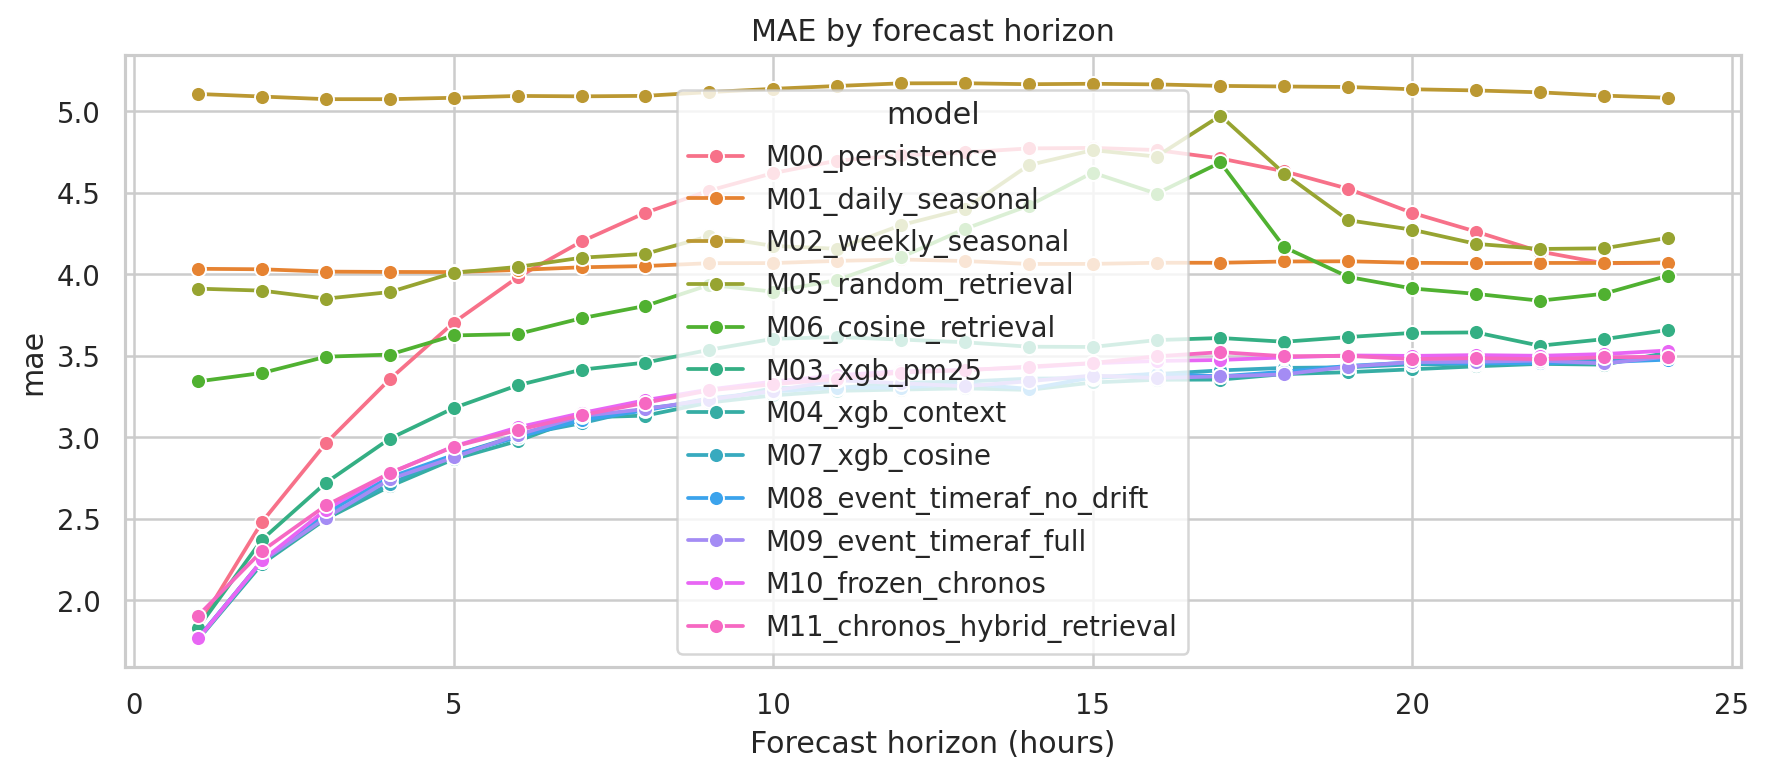
\includegraphics[width=\columnwidth]{figures/mae_by_horizon.png}
\caption{MAE by forecast horizon for the final test run.}
\label{fig:mae_horizon}
\end{figure}

\begin{figure}[!t]
\centering
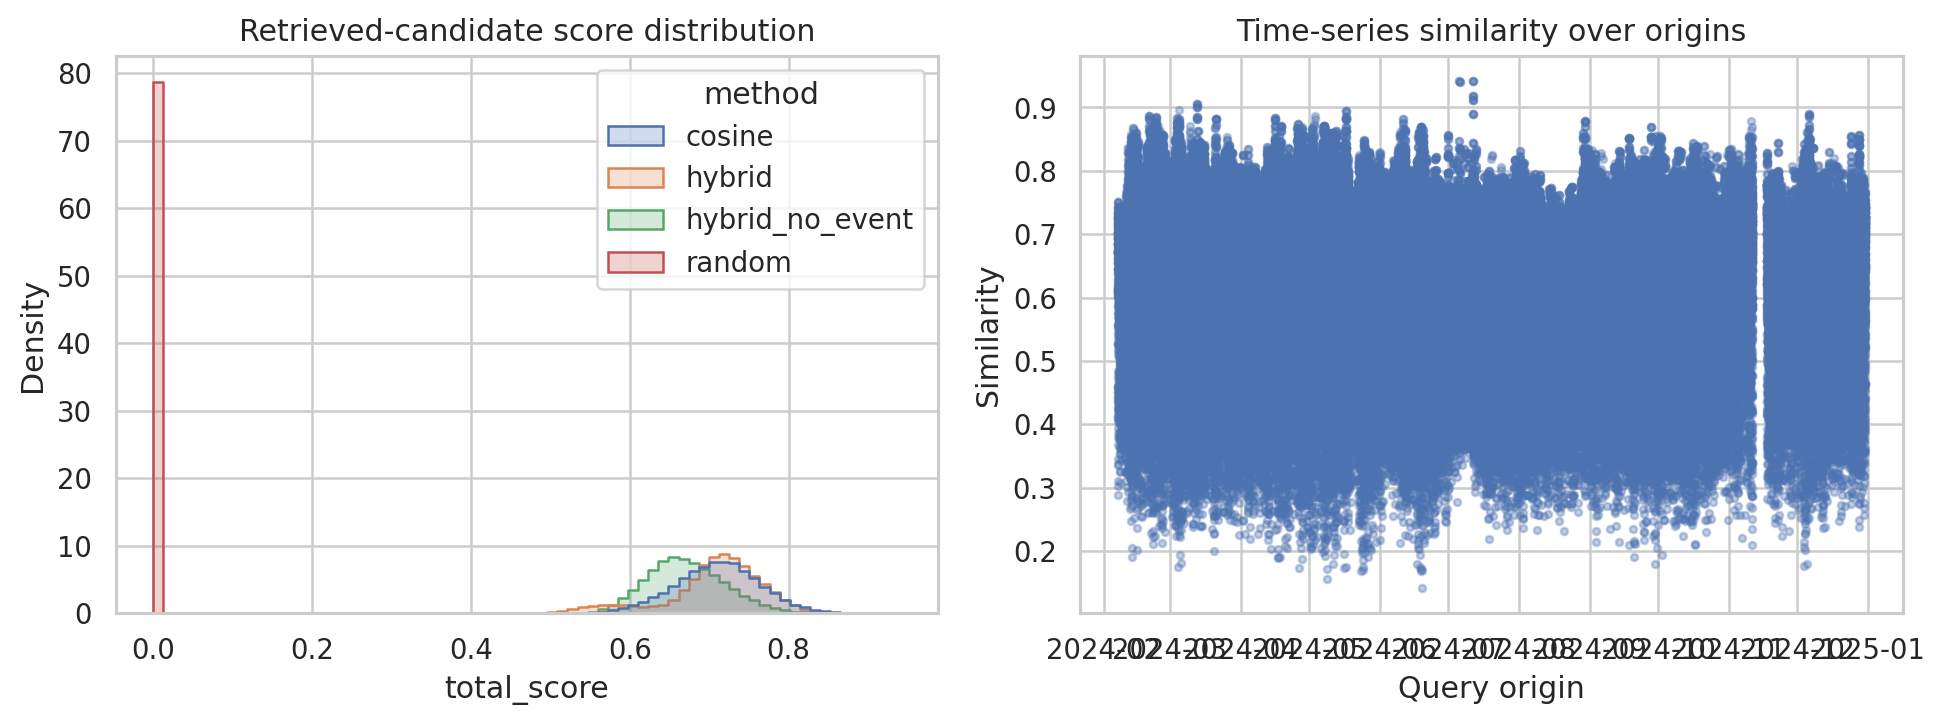
\includegraphics[width=\columnwidth]{figures/retrieval_diagnostics.png}
\caption{Retrieval diagnostics for the final test run.}
\label{fig:retrieval_diagnostics}
\end{figure}

\begin{figure}[!t]
\centering
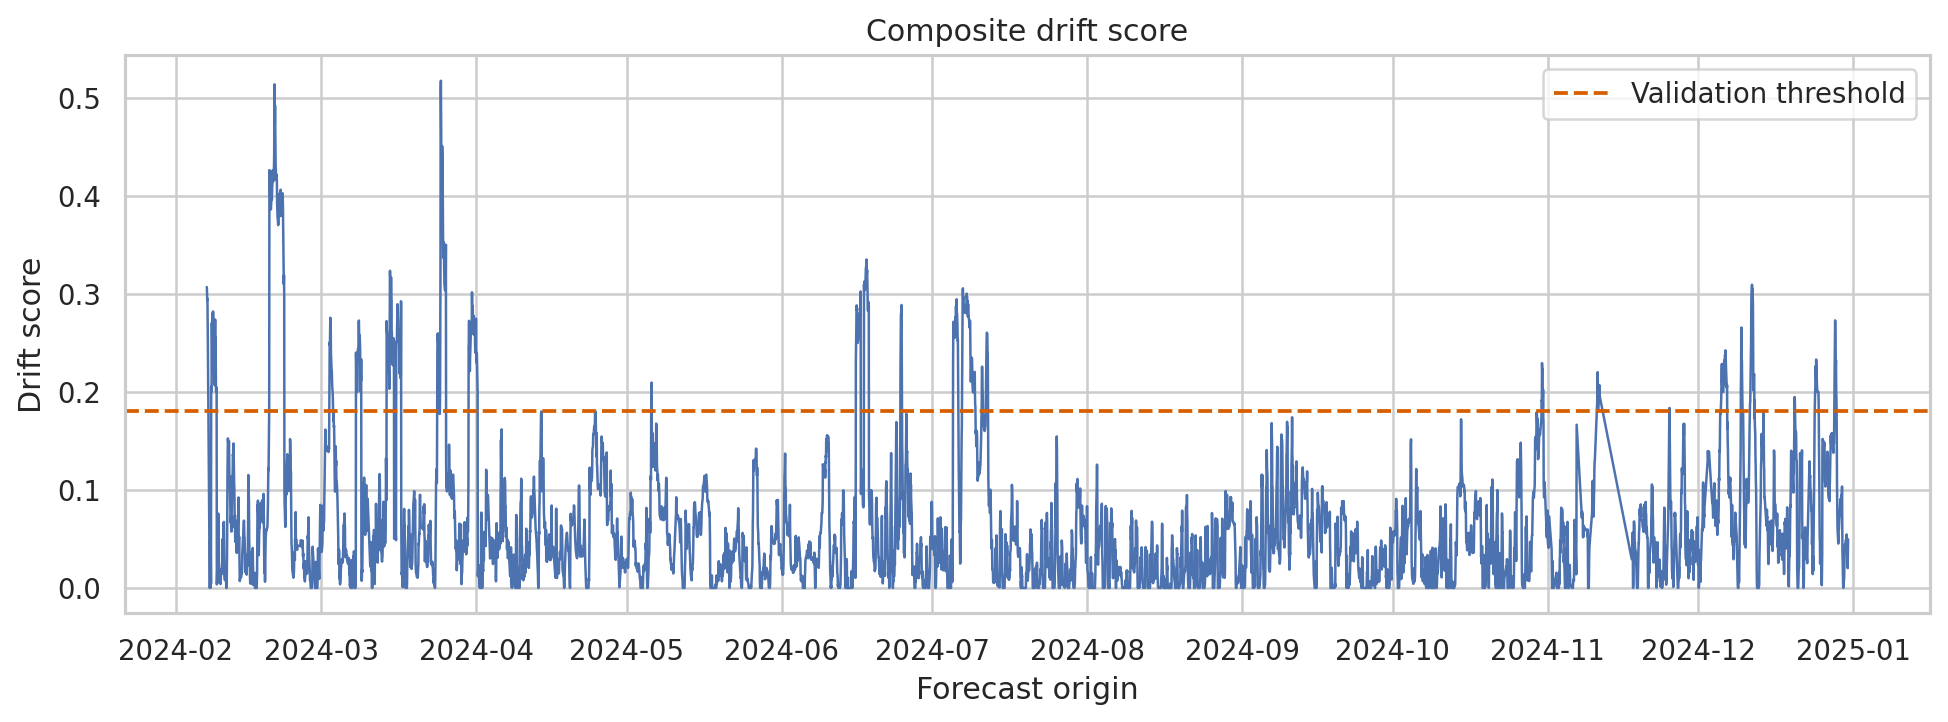
\includegraphics[width=\columnwidth]{figures/drift_scores.png}
\caption{Drift-score diagnostics for the final test run.}
\label{fig:drift_scores}
\end{figure}

The main interpretation is that conventional supervised context features are
very strong for this Los Angeles County 24-hour PM2.5 task. Retrieval is useful
as a standalone historical-pattern baseline and gives a small favorable MSE
change when fused with frozen Chronos-Bolt, but the present feature-level
Event-TimeRAF design does not beat the best XGBoost context baseline overall.
This negative result is important for the final paper: Event-TimeRAF should be
presented as an implemented and audited event-aware retrieval framework with
mixed empirical effects, not as a uniformly superior forecasting model.

Finally, all event-aware interpretations must be read with the availability
caveat. NOAA Storm Events records are official and hash-verified, but the source
does not provide machine-readable publication timestamps. The experiment records
event start as the availability time, so event-related results are retrospective
sensitivity results. A strict operational study would require event or smoke
sources with genuine issue or publication times, such as an audited NOAA HMS
cache or alert product archive.

\section{Conclusion}

This draft proposed Event-TimeRAF, an event-aware retrieval-augmented framework for explainable Los Angeles County PM2.5 forecasting under distribution shift. The proposed framework extends the TimeRAF idea by combining time-series retrieval with weather, calendar, source-recorded environmental events, drift indicators, and evidence-based explanation generation. The implementation is designed as a Kaggle-compatible pipeline using official US data, direct XGBoost baselines, leakage-safe retrieval, and a frozen-TSFM publication gate.

Because the complete experiment has not yet been executed, this manuscript does not report performance claims. The next step is to run and audit the full 2019--2024 pipeline on Kaggle, complete the frozen-TSFM publication gate, freeze validation choices, evaluate the test set once, and populate the paper only from saved artifacts. The conclusion will be revised after those results are available.


\bibliographystyle{IEEEtran}
\bibliography{references}

\end{document}
